\documentclass[a4paper]{article}
\usepackage{amsmath}
\usepackage{fancyhdr}
\usepackage{graphicx}
\pagestyle{fancy}
\lfoot{Andrew Martin}
\rfoot{10/8/2017}
\begin{document}
	\title{SMI Assignment 1}
	\date{August 10, 2017}
	\author{Andrew Martin}
	\maketitle
	
	Question 1:\\
	$(Y_i)_{i=1}^n$ are i.i.d $N(\mu,\sigma^2)$ r.vs with sample mean $\bar{Y}$.\\
	
	a) Find $E\left[\bar{Y}^2\right]$\\
	$$var(\bar{Y})=E\left[\bar{Y}^2\right]-E\left[\bar{Y}\right]^2$$
	$$\implies E\left[\bar{Y}^2\right]=var(\bar{Y})+E\left[\bar{Y}\right]^2$$
	
	$$=var(\frac{1}{n}\sum_{i=1}^{n}Y_i)+E\left[\frac{1}{n}\sum_{i=1}^{n}Y_i\right]^2$$
	$$=\frac{1}{n^2}\sum_{i=1}^{n}var(Y_i)+\frac{1}{n^2}E\left[\sum_{i=1}^{n}Y_i\right]^2$$
	$$=\frac{1}{n^2}\sum_{i=1}^{n}\sigma^2+\frac{1}{n^2}(\sum_{i=1}^{n}E\left[Y_i\right])^2$$
	$$=\frac{n}{n^2}\sigma^2+\frac{1}{n^2}(\sum_{i=1}^{n}\mu)^2$$
	$$=\frac{\sigma^2}{n}+\mu^2$$

	
	
	
	
	b) For each \textit{i} with $1\leq i\leq n$, prove $\bar{Y}$ and $Y_i - \bar{Y}$ are uncorrelated\\
	$$cov(\bar{Y},Y_i-\bar{Y})=E\left[(\bar{Y}-E[\bar{Y}])((Y_i-\bar{Y})-E[Y_i-\bar{Y}])\right]$$
	$$=E\left[(\bar{Y}-E[\bar{Y}])((Y_i-\bar{Y})-E[Y_i]-E[\bar{Y}])\right]$$
	From above $E[\bar{Y}] =\mu$, so:
	$$=E\left[(\bar{Y}-\mu)((Y_i-\bar{Y})-\mu-\mu)\right]$$
	$$=E\left[(\bar{Y}-\mu)(Y_i-\bar{Y})\right]$$
	$$=E[\bar{Y}Y_i-Y_i\mu +\mu \bar{Y}-\bar{Y}^2]$$
	$$=E[\bar{Y}Y_i]-E[Y_i\mu] +E[\mu \bar{Y}]-E[\bar{Y}^2]$$
	$$=E[\bar{Y}Y_i]-\mu E[Y_i] +\mu E[\bar{Y}]-\frac{\sigma^2}{n}-\mu^2$$
	But From Tute 1: $E[\bar{Y}Y_i]=\frac{-\sigma^2}{n}+\mu^2$, so:
	$$=\frac{-\sigma^2}{n}+\mu^2-\mu E[Y_i] +\mu E[\bar{Y}]-\frac{\sigma^2}{n}-\mu^2$$
	$$=-\mu \mu +\mu \mu=0$$
	Therefore they are uncorrelated.
	
	\newpage
	Question 2:\\
	$(Z_i)_{i=1}^p$ are i.i.d $N(0,1)$ random variables with
	$$X=\sum_{i=1}^{p}Z_i^2$$
	
	a) Find the moment generating function and distribution of X, assuming $M_{Z^2}(t)=(1-2t)^{-1/2}$, where $Z${\raise.17ex\hbox{$\scriptstyle\mathtt{\sim}$}} $N(0,1)$
	$$M_X(t)=E\left[e^{tX}\right]=E\left[e^{t\sum_{i=1}^{p}Z_i^2}\right]$$
	Note that
	$$M_{Z^2}(t)=E[e^{tZ^2}]=E[e^te^{Z^2}]=(1-2t)^{-1/2}$$
	So:
	$$M_X(t)=E\left[e^te^{\sum_{i=1}^{p}Z_i^2}\right]$$
	$$=E\left[e^t\prod_{i=1}^{p}e^{Z_i^2}\right]$$
	Since $Z_i$ are i.i.d
	$$=\prod_{i=1}^{p}E\left[e^{tZ_i^2}\right]$$
	$$=\prod_{i=1}^{p}M_{Z^2}(t)$$
	$$=\prod_{i=1}^{p}(1-2t)^{-1/2}$$
	
	
	b) $(Y_i)_{i=1}^p$ are independent normal random variables with different means and variances\\
	i.e. \\$Y_i${\raise.17ex\hbox{$\scriptstyle\mathtt{\sim}$}} $N(\mu_i,\sigma^2_i), i=1,...,p$\\
	Show that 
	$W=\sum_{i=1}^{p}\frac{(Y_i-\mu_i)^2}{\sigma_i^2}${\raise.17ex\hbox{$\scriptstyle\mathtt{\sim}$}}$\chi_p^2$\\
	where $\chi_p^2$ denotes the chi-squared dist with \textit{p} degrees of freedom.
	$$W=\sum_{i=1}^{p}\frac{(Y_i-\mu_i)^2}{\sigma_i^2}$$
	Note that $\frac{(Y_i-\mu_i)}{\sigma_i}${\raise.17ex\hbox{$\scriptstyle\mathtt{\sim}$}}$Z${\raise.17ex\hbox{$\scriptstyle\mathtt{\sim}$}}$N(0,1)$
	So from this:
	$$W=\sum_{i=1}^{p}\frac{(Y_i-\mu_i)}{\sigma_i}=\sum_{i=1}^{p}Z_i^2$$
	For which, the MGF is as above: $=\prod_{i=1}^{p}(1-2t)^{-1/2}$\\
	Which is the form of a $\chi^2$ MGF 
	
	
	
	\newpage
	Question 3\\
	Let $X${\raise.17ex\hbox{$\scriptstyle\mathtt{\sim}$}}$Bin(n,p)$\\
	And
	$\hat{p}^2=\left(\frac{X}{n}\right)^2$\\
	
	a) Find $E\left[\hat{p}^2\right]$ and state the bias\\
	$$E[\hat{p}^2]=E[(\frac{X}{n})^2]$$
	$$\implies E\left[(\frac{X}{n})^2\right]=var(\frac{X}{n^2})+E\left[\frac{X}{n}\right]^2$$
	$$=\frac{1}{n^2}var(X)+\frac{1}{n^2}E\left[X\right]^2$$
	$$=\frac{1}{n^2}np(1-p)+\frac{1}{n^2}(np)^2$$
	$$=\frac{p(1-p)}{n}+p^2$$
	$$=\frac{p-p^2+np^2}{n}$$
	
	The bias is: $$\frac{p-p^2}{n}$$
	
	
	
	b) Show that
	$$E\left[\frac{\hat{p}(1-\hat{p})}{n-1}\right]=\frac{p(1-p)}{n}$$
	Start with the left hand side:
	$$E\left[\frac{\hat{p}(1-\hat{p})}{n-1}\right]=\frac{1}{n-1}E\left[\hat{p}(1-\hat{p})\right]$$
	$$=\frac{1}{n-1}E\left[\hat{p} -\hat{p}^2\right]$$
	$$=\frac{1}{n-1}(E[\hat{p}] -E[\hat{p}^2])$$
	$$=\frac{1}{n-1}\left(E[\frac{X}{n}]-(\frac{p-p^2+np^2}{n})\right)$$
	$$=\frac{1}{n^2-n}\left(E[X]-(p-p^2+np^2)\right)$$
	$$=\frac{1}{n^2-n}\left(np-p+p^2-np^2\right)$$
	$$=\frac{1}{n^2-n}\left(p(n-1+p-np)\right)$$
	$$=\frac{n-1}{n^2-n}\left(p(1-p)\right)$$
	$$=\frac{p(1-p)}{n}$$
	
	
	c) Using a) and b) find an unbiased estimator for $p^2$.\\
	If T is an estimator for $\theta$ then the bias is: $b_T (\theta) = E[T] - \theta$. For unbiased, set this to zero.\\
	I.e. In this case, $b_T (p^2) = E[T]-p^2=0$\\
	So aim to find T such that $E[T]=p^2$
	By subtracting the expectations in a) and b)
	$$E[\hat{p}^2]-E\left[\frac{\hat{p}(1-\hat{p})}{n-1}\right]$$
	$$=\frac{p-p^2+np^2}{n}-\frac{p(1-p)}{n}$$
	$$=\frac{np^2}{n}$$
	$$=p^2$$
	So an unbiased estimator, T, for $p^2$, would be:
	$$T=\hat{p}^2-\frac{\hat{p}(1-\hat{p})}{n-1}$$
	
	\newpage
	Question 4\\
1) Clean all the variables (include code)\\
2) Produce an appropriate plot for each variable\\
i.e for categorical - bar chart, for quantitative - histogram.\\
Label and caption each of these\\
3) For the quantitative variables, identify if they are: unimodal or bimodal, whether it is symmetric, left-skewed or right-skewed. For categorical, identify the most common level\\
	
Price\\
Cross\\
Pet offered by\\
Microchip\\
Vaccination\\
Desexing status\\
Relinquished or not\\

The R code is attached and will be referenced from here, onwards.\\

\noindent{
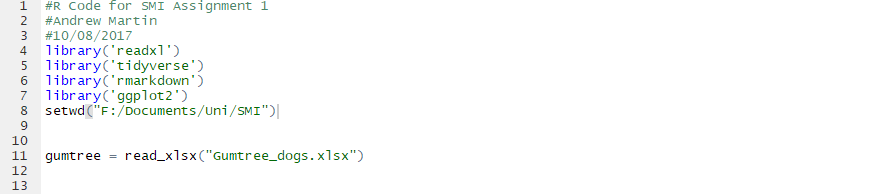
\includegraphics[scale=.75]{gumtree_1.PNG}\\
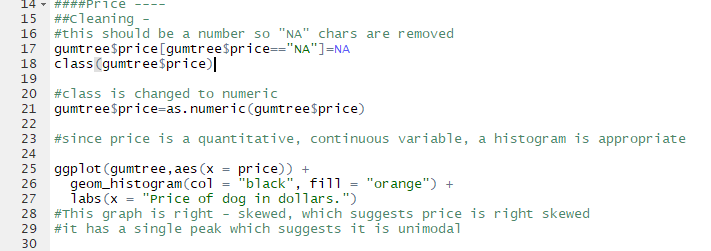
\includegraphics[scale=.75]{gumtree_PriceCode.PNG}\\
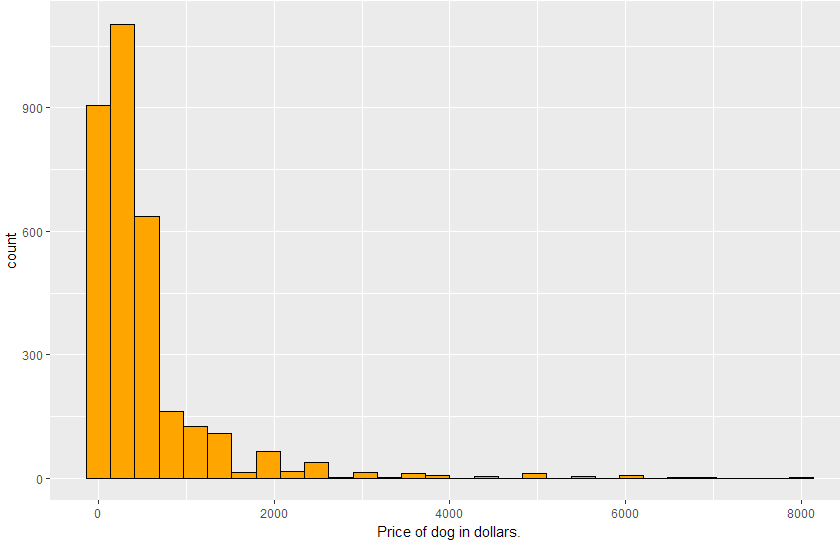
\includegraphics[scale=.75]{gumtree_PriceGraph.PNG}\\
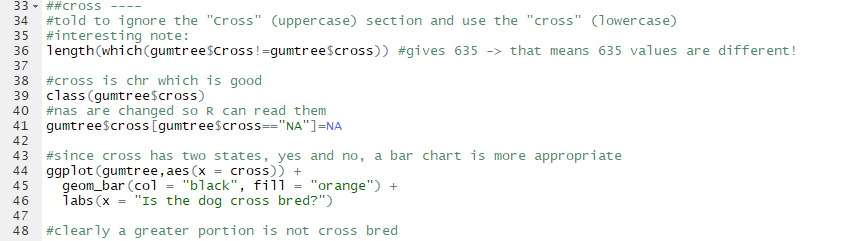
\includegraphics[scale=.75]{gumtree_CrossCode.PNG}\\
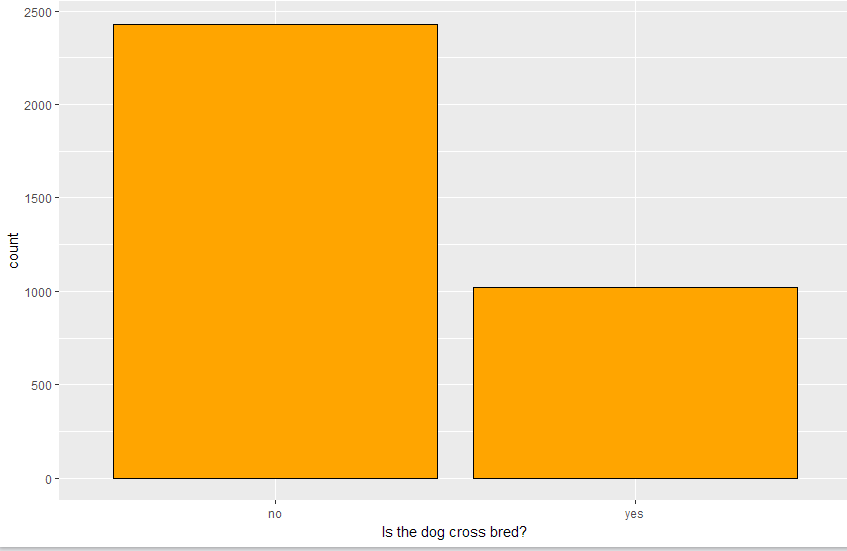
\includegraphics[scale=.75]{gumtree_CrossGraph.PNG}\\
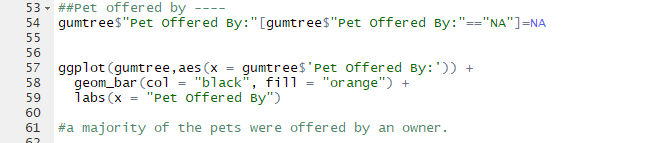
\includegraphics[scale=.75]{gumtree_SellerCode}\\
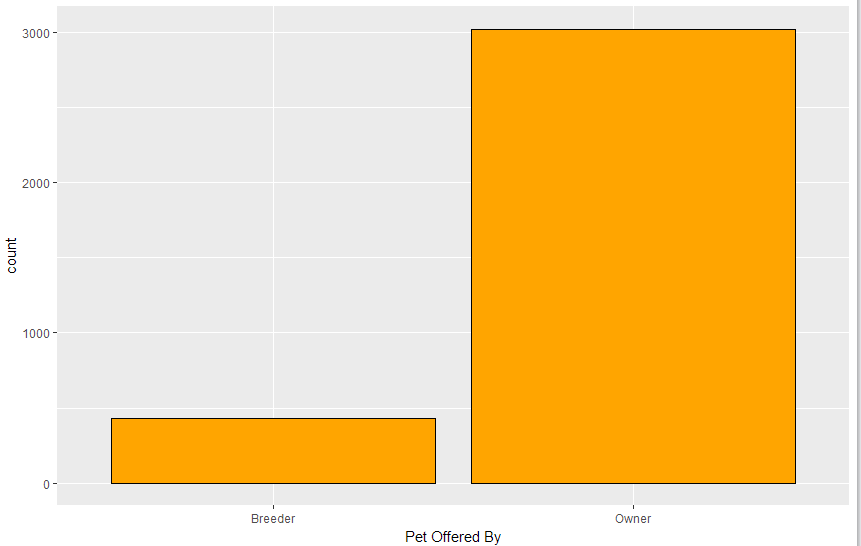
\includegraphics[scale=.75]{gumtree_SellerGraph.PNG}\\
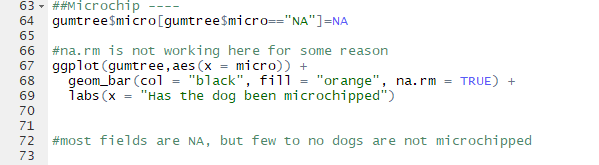
\includegraphics[scale=.75]{gumtree_MicroCode.PNG}\\
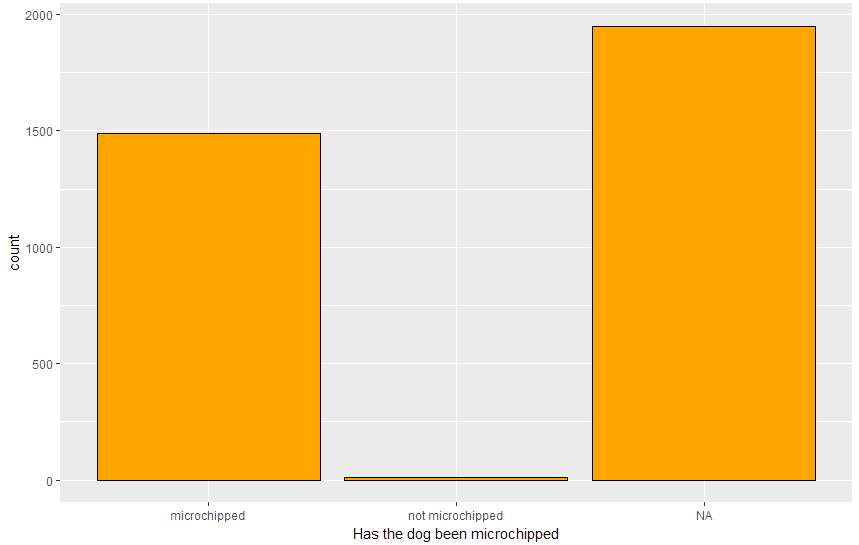
\includegraphics[scale=.75]{gumtree_MicroGraph.PNG}\\
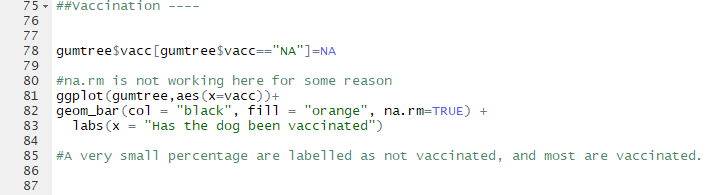
\includegraphics[scale=.75]{gumtree_VaccCode.PNG}\\
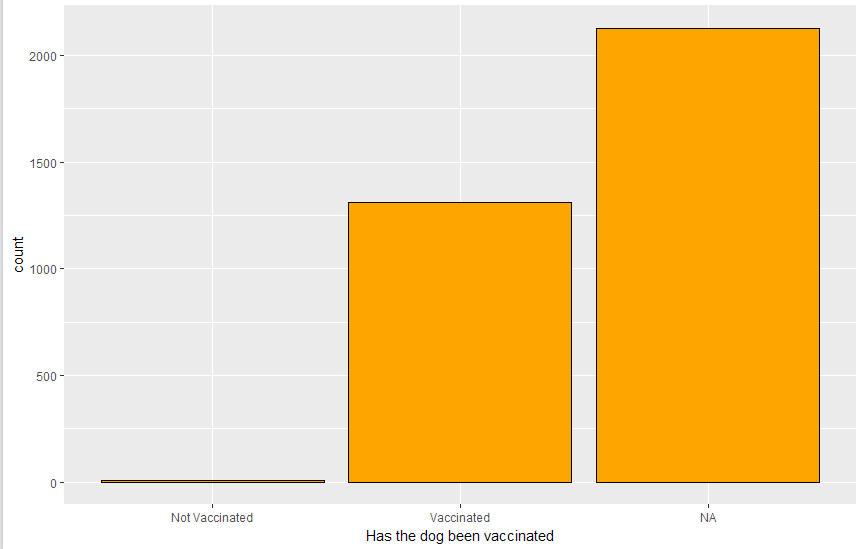
\includegraphics[scale=.75]{gumtree_VaccGraph.PNG}\\
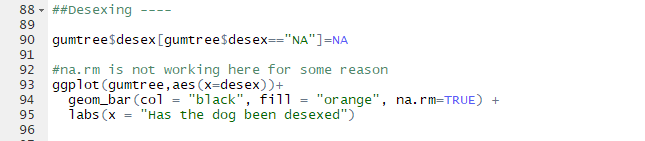
\includegraphics[scale=.75]{gumtree_DesexCode.PNG}\\
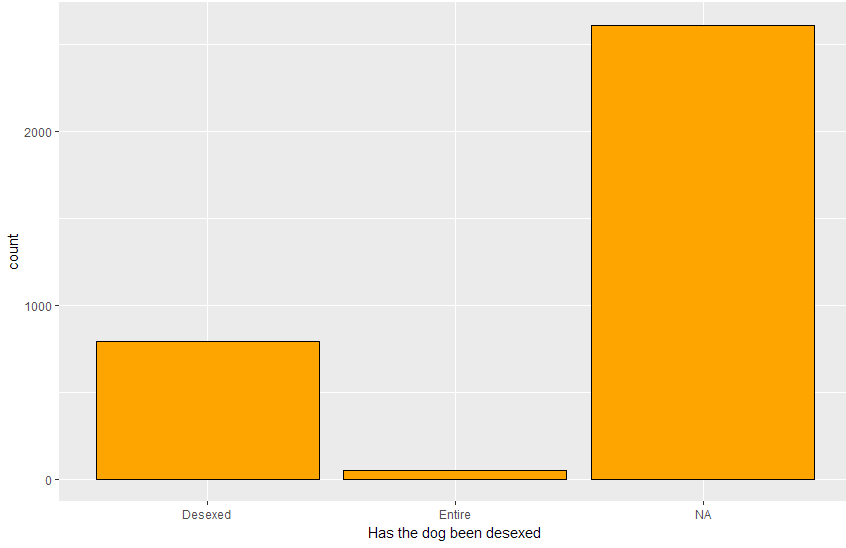
\includegraphics[scale=.75]{gumtree_DesexGraph.PNG}\\
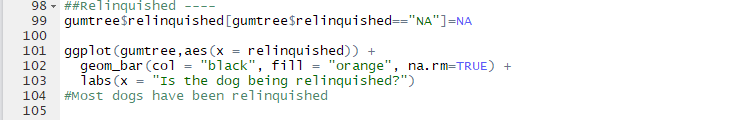
\includegraphics[scale=.75]{gumtree_RelinCode.PNG}\\
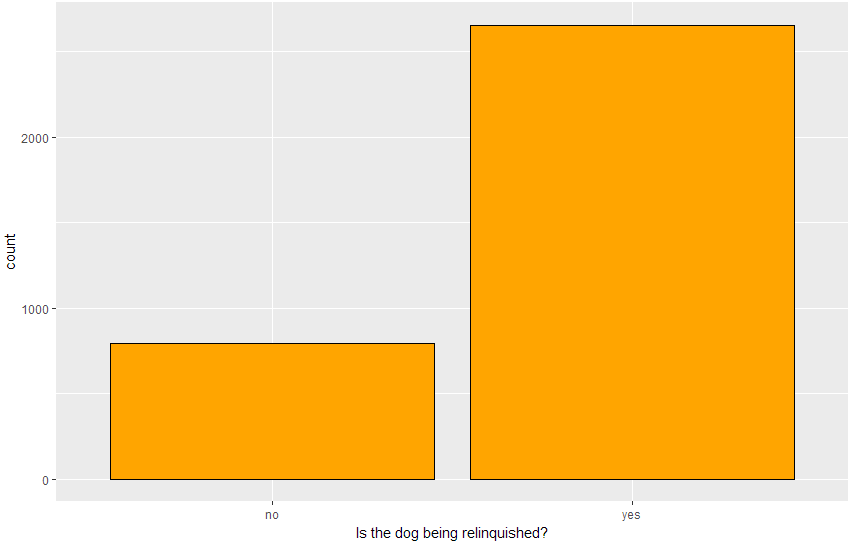
\includegraphics[scale=.75]{gumtree_RelinGraph.PNG}\\}


	
	
\end{document}